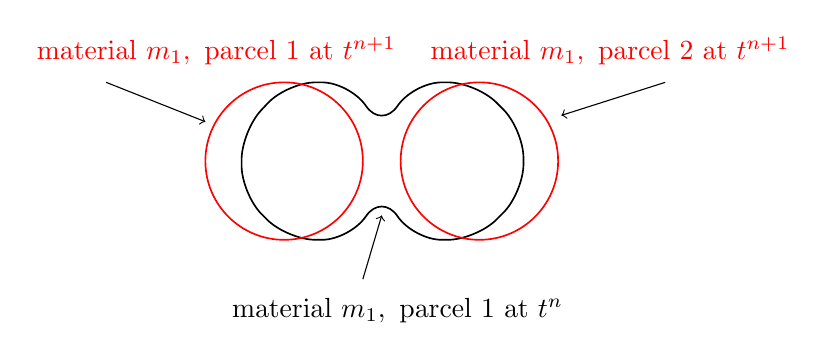
\begin{tikzpicture}

 \draw[rounded corners=10.33pt, semithick] (0.8,3) -- (0.22,2.38) -- (0.22,1.58) -- (0.8,1) -- (1.6,1) -- (2,1.6) -- (2.4,1) -- (3.2,1) -- (3.8,1.6) -- (3.8,2.4) -- (3.2,3) -- (2.4,3) -- (2,2.4) -- (1.6,3) -- cycle;


  \draw[red, semithick] (0.76,2) circle (1cm);
  \draw[red, semithick] (3.24,2) circle (1cm);



\node at (2.2,0.1){$\textcolor{black}{ \mbox{material } m_{1},\mbox{ parcel } 1 \mbox{ at } t^{n}}$};



\node at (-0.1,3.4){$\textcolor{red}{ \mbox{material } m_{1},\mbox{ parcel } 1 \mbox{ at } t^{n+1}}$};


\node at (4.9,3.4){$\textcolor{red}{ \mbox{material } m_{1},\mbox{ parcel } 2 \mbox{ at } t^{n+1}}$};







  \draw[->] (1.76,0.5) -- (2,1.31);
  \draw[->] (-1.5,3) -- (-0.24,2.5);
  \draw[->] (5.6,3) -- (4.28,2.58);
\end{tikzpicture}2